Due to the reasons which we have discussed in the section \ref{sec:StateOfTheArt}, the type of the detector which we have developed in order to measure the tritium that there is in water samples is a scintillator detector. It consists in a chain of three main elements:

\begin{itemize}

\item{} The scintillator, that is the material in charge of detecting the tritium event. The tritium particle or a general particle (ionizing radiation) hit this material and deposits part of their kinetic energy (or all, as in the case of the tritium event) in it through ionization and excitation. Part of this energy deposited is converted in photons, in our case in the visible range.

The number of photons produced carry information about the particle detected, such as its energy, type, etc.

\item{} The photosensor, which is the part of the detector in charge of detecting the photons produced by the scintillator that reach its sensitive element (the more scintillated photons arrive to your photosensor, the better signal you have in your detector). 

The most used photosensor in nuclear physics are SiPMs and PMTs which detects some of the photons produced in the scintillator and transforms it in electrons which are multiplied with a factor of around $10^6$. This millions of electrons form a electronic pulse whose properties has information of the photons that has been detected.

\item{} The electronic system, which is the part of the scintillator detector in charge of processesing and analyzing (first analogically and then digitally) this electrical pulse of the photosensor to give us useful information about the event detected that we can understand and interpret such as a number, for instance the activity, or some kind of spectrum like energetic spectrum.

\end{itemize}

In figure \ref{fig:ScintillatorDetector} we can see the scheme of a scintillation detector where the scintillator material detects ionizing radiation and produces photons that will be guided by the reflector and the light guide to the photosensor. There, some of the photons that reach the sensible part of the photosensors will be converted and multiplied into millions of electrons that will form a electronic pulse. The output signal of the photosensor (electronic pulse) will be processed and analyzed by the corresponding electronics:

\begin{figure}[hbtp]
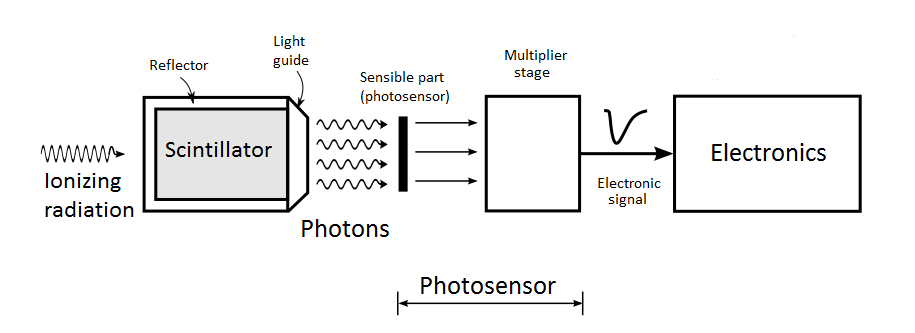
\includegraphics[scale=0.6]{3DesignPrinciples/ScintillatorDetector.png}
\centering
\caption{Scheme of the scintillator detector \cite{CentelleadoresEspanyol}\label{fig:ScintillatorDetector}}
\end{figure}